% !TEX TS-program = XeLaTeX
% Commands for running this example:
% 	 xelatex twocol-example
% 	 xelatex twocol-example
% End of Commands
\documentclass[twocolumn]{article}
\pagestyle{empty}

\usepackage{tram}
\usepackage{relsize}
\usepackage{amsmath}
\usepackage{float}

\usepackage{xepersian}
\settextfont[Scale=1]{B Nazanin}
%\setlatintextfont{serif}


\newcommand\numberthis[1][]{%
    \refstepcounter{equation}%
    \ifx#1\empty\else\label{eq:#1}\fi%
    \tag{\theequation}%
}
\newcommand{\enfootnote}[1]{\footnote{\lr{#1}}}

\title{ 
\Large{
\textbf{
تشخیص ناهنجاری در فضاهای با مقیاس بزرگ و ابعاد بالا با استفاده از مدل ترکیبی ماشین بردار پشتیبان تک کلاسه و یادگیری عمیق
}}}
\date{
\small{
\textbf{
آبان ماه 1395
}}}
\author{
\small{
\textbf{
احمد اسدی - ۹۴۱۳۱۰۹۱
}}}

\begin{document}
\twocolumn[
  \begin{@twocolumnfalse}
    \maketitle
    \begin{abstract}
{\centering
\vspace{10pt}
\begin{tram}[400]
\parbox{\textwidth}{%
تشخیص ناهنجاری در مسائلی که با داده‌های با ابعاد بالا روبرو هستند با چالش‌های مختلفی روبرو است. یکی از مهم‌ترین این چالش‌ها، مشکل «نفرین ابعاد» است. با افزایش تعداد ابعاد مورد استفاده در مساله، تعداد ویژگی‌های استخراج شده که ارتباط معناداری با برچسب داد‌ه‌ها ندارند، افزایش خواهد یافت. این مساله باعث ایجاد مشکلات متعددی در مسیر تشخیص ناهنجاری در فضاهای با بعد بالا می‌شود. برای حل این مشکل، می‌توان با استفاده از روش‌های مبتنی بر خوشه‌بندی، ابتدا ویژگی‌های مناسبی را از بین تمام ویژگی‌های موجود انتخاب کرد به طوری‌ که علاوه بر کاهش ابعاد مساله، توانایی مناسبی در ایجاد توزیع‌های خوش‌فرم دربرچسب‌های مختلف را نیز داشته باشند. سپس با استفاده از این‌ ویژگی‌ها و الگوریتم‌های معمول در حوزه تشخیص ناهنجاری، عملیات مورد نظر را اجرا نمود. در این پژوهش، در مرحله اول با استفاده از یک شبکه عصبی باور عمیق، ویژگی‌های مناسب استخراج شده و سپس با به‌کارگیری یک مدل ماشین بردار پشتیبان تک کلاسه در مرحله دوم، عملیات دسته‌بندی انجام می‌شود.
}
\end{tram}
}
    \end{abstract}
  \end{@twocolumnfalse}
]

\section{مقدمه}
استخراج ویژگی‌ برای داده‌ها از جمله مهم‌ترین چالش‌ها در فرآیند حل مساله است. علاوه بر این، در شرایطی که تعداد داده‌ها بسیار زیاد باشد، عدم وجود داده‌های برچسب خورده به اندازه کافی، لزوم استفاده از یادگیری بدون نظارت را بیش از پیش جلوه می‌دهد. هدف اصلی در پژوهش‌های مربوط به تشخیص ناهنجاری این است که داده‌هایی را که رفتاری غیر عادی نسبت به داده‌های دیگر از خود نشان می‌دهند، شناسایی شوند. چالش اصلی در تشخیص ناهنجاری، توانایی کنترل مناسب مجموعه‌دادگان بزرگ و نویزی است. در پژوهش مورد مطالعه
\cite{erfani2016high}
، با ارائه یک روش ترکیبی بدون نظارت، سعی می‌شود تا حد ممکن بر این مشکلات غلبه شود.
\\
مجموعه‌های دادگان ابعاد بالا، مشکلاتی برای تشخیص ناهنجاری ایجاد می‌کنند که از جمله مهم‌ترین آن‌ها می‌توان به ۱) افزایش نمایی فضای جستجو، ۲) وجود ویژگی‌های نامربوط به برچسب‌ها. مدل‌های مختلفی برای حل این مساله ارائه شده است. یکی از مشهورترین این مدل‌ها، دسته مدل‌های موسوم به ماشین‌های بردار پشتیبان تک کلاسه\enfootnote{One Class SVMs} هستند. این دسته از مدل‌ها سعی در مدل‌سازی توزیع داده‌های عادی موجود در مجموعه داده‌ها دارند و به طور همزمان سعی می‌کنند تا حد ممکن، مدل ارائه شده را نسبت به داده‌های نویزی یا ناهنجاری‌های موجود، غیرحساس کنند. به همین منظور، با استفاده از یک تابع هسته\enfootnote{Kernel Function} داده‌های موجود را به یک فضای با ابعاد بالاتر نگاشت می‌کنند به طوری‌که بتوان در فضای جدید، داده‌های عادی را به راحتی از ناهنجاری‌ها جدا نمود. 
\\
از جمله مزایای این دسته از مدل‌ها می‌توان به سه مورد زیر اشاره کرد:
\begin{enumerate}
\item قدرت تعمیم‌پذیری بسیار بالا
\item عدم وجود مشکل اکسترمم‌های محلی
\item قدرت مدل‌سازی هر مجموعه‌داده‌ای بسته به نوع تابع هسته تعریف شده
\end{enumerate}
با وجود این‌که ماشین‌های بردار پشتیبان مزایای زیادی دارند، محدودیت‌هایی که در مسائل ایجاد می‌کنند باعث می‌شود نتوان از آن‌ها مستقیما در مسائل با مقیاس بزرگ و ابعاد بالا به خوبی استفاده کرد. از جمله این محدودیت‌ها، رابطه نمایی زمان اجرای این الگوریتم‌ها با تعداد رکوردهای موجود در مجموعه‌داده است. از طرفی با توجه به مشکل «نفرین ابعاد» با افزایش بعد مساله باید تعداد داده‌های آموزشی به طور نمایی افزایش یابد که باعث می‌شود نتوان از ماشین‌های بردار پشتیبان در مسائل با ابعاد بالا استفاده نمود.
\\
یکی از مدل‌های مطرح در زمینه دسته‌بندی و کاهش بعد، شبکه‌های باور عمیق هستند. این شبکه‌ها با استفاده از یک الگوریتم حریصانه، به شکل لایه به لایه آموزش داده‌ می‌شوند و قادرند در مسائل دسته‌بندی چندکلاسه عملکردهای بسیار مناسبی از خود نشان بدهند. 
\\
از مزایای شبکه باور عمیق می‌توان به قابلیت بالای این شبکه در مدل‌سازی داده‌ها با ابعاد بالا و مقیاس بزرگ اشاره کرد. همین‌طور این شبکه‌ها قادرند داده‌های پیچیده و با ابعاد بالا را تحت یک روش بدون نظارت، در یک فضای با ابعاد کوچکتر (یا بزرگتر) بازتولید کنند.
\\
با وجود مزایای ذکر شده، شبکه‌های باور عمیق دچار یک ضعف اساسی هستند و آن این است که تابع هدف این شبکه‌ها عموما غیر محدب است. این مساله باعث به وجود آمدن اکسترمم‌های محلی در تابع هدف می‌شود. وجود اکسترمم‌های محلی در تابع هدف به معنی عدم وجود تضمین برای بهینه بودن پاسخ تابع است.
\\
با در نظر گرفتن معایب مدل ماشین بردار پشتیبان در حوزه تشخیص ناهنجاری در فضاهای بزرگ و ابعاد بالا و مزایایی که با استفاده از شبکه‌های باور عمیق می‌توان به آن‌ها دست یافت، مدل مرکبی از این دو روش در پژوهش مورد مطالعه ارائه شده است که بهبودهای مناسبی نسبت به روش‌های ارائه شده دیگر از خود نشان می‌دهد.
\\
از‌ آنجا که در پژوهش مورد مطالعه، از دو روش مختلف موسوم به بردار پشتیبان توصیف‌گر داده 
\enfootnote{SVDD}
\cite{tax2004support}
 و ماشین بردار پشتیبان خطی 
\enfootnote{PSVD}
\cite{scholkopf2001estimating}
 استفاده شده است و توضیحات جامعی درباره آن‌ها ارائه نشده، در این گزارش، ابتدا هر یک از این روش‌ها را از مقالات اصلی که در آن ارائه شده‌اند مورد بررسی قرار می‌دهیم و در نهایت به بررسی روش ارائه شده در این پژوهش و نتایج این روش‌ها خواهیم پرداخت.

\section[بردار پشتیبان توصیف‌گر داده]{بردار پشتیبان توصیف‌گر داده\cite{tax2004support}}
در این پژوهش، هدف اصلی یافتن یک محدوده\enfootnote{Boundary} برای داده‌ها است به طوری‌که علاوه بر دربر گرفتن داده‌ها، فضای اضافی اشغال نکند. به این ترتیب با تشکیل محدوده مورد نظر برای داده‌ها، داده‌هایی که در محدوده قرار نمی‌گیرند به عنوان ناهنجاری شناخته شده و گزارش می‌شوند. برای به‌دست‌ آوردن چنین محدوده‌ای از روش‌های بهینه‌سازی ریاضیاتی برای ارضای هر دو محدودیت استفاده شده است که در این بخش به بررسی آن خواهیم پرداخت.\\
فرض می‌کنیم بردار $x_i$ یک بردار ستونی است که نشان‌دهنده یکی از داده‌های موجود در مجموعه‌داده است. همین‌طور فرض می‌کنیم $x^2 = x \cdot x$.
\\
برای شروع باید یک مدل پایه به عنوان محدوده مورد نظر فرض نمود. در این روش از یک \textbf{ابرکره} به عنوان مدل پایه استفاده می‌شود. پارامترهای مربوط به یک ابرکره، شامل شعاع آن $R > 0$ و نقطه مرکز آن $a$ می‌شود. برای محدود کردن فضای اشغال شده توسط ابر کره، می‌توان مقدار $R^2$ را کمینه کرد با این محدودیت که ابرکره باید بتواند تمام داده‌ها را شامل شود. برای ارضای محدودیت شامل‌ شدن تمام نقاط مجموعه‌داده، می‌توان عبارت $||x_i - a||^2 \leq R^2$  را به ازای تمام $i$ها، به عنوان یکی از قیود مساله، مورد نظر قرار داد.
\\
با توجه به این‌ که داده‌های موجود در این مسائل شامل داده‌های نویز و ناهنجاری‌ها هستند، نباید محدودیت شمول در ابرکره،‌ به شکل یک محدودیت اکید باشد. برای حل این مساله از متغیر‌های کمکی\enfootnote{Slack Variable} $\zeta_i \geq 0$ استفاده نموده و فرم تابع کمینه‌کننده را به شکل $R^2 + C\mathlarger{\Sigma_i}\zeta_i$ تغییر می‌دهیم که در آن، متغیر $C$ یک متغیر کنترل‌کننده است که با استفاده از آن می‌توان میزان اهمیت دو محدودیت را نسبت به هم کنترل کرد.  همین‌طور محدودیت شمول به شکل $||x_i - a||^2 \leq R^2 + \zeta_i$ تغییر می‌کند که در آن $\forall i, \zeta_i \geq 0$ است.
\\
در نهایت می‌توان تمام موارد گفته شده را با استفاده از ضرایب لاگرانژ به فرم رابطه
\eqref{eq:1}
 نوشت.


\begin{align*}
L(R, &a, \alpha_i, \gamma_i, \zeta_i) = \\
&R^2 + C\mathlarger{\Sigma_i}\zeta_i \\
&-\mathlarger{\Sigma_i} \alpha_i (R^2 + \zeta_i -(|x_i|^2 - 2 a\cdot x_i + ||a||^2) ) \\
&-\mathlarger{\Sigma_i}\gamma_i \zeta_i
\numberthis
\label{eq:1}
\end{align*}

رابطه $L$ باید نسبت به متغیرهای $R$، $a$ و $\zeta_i$ بیشینه و نسبت به ضرایب لاگرانژ $\alpha_i$ و $\gamma_i$ کمینه شود. با مشتق‌گیری از $L$ خواهیم داشت:

\begin{align*}
\frac{\partial L}{\partial R} &= R(2 - 2\mathlarger{\Sigma_i}\alpha_i) = 0 \rightarrow \mathlarger{\Sigma_i} \alpha_i = 1 
\numberthis
\label{eq:2}
\end{align*}

\begin{align*}
\frac{\partial L}{\partial a} &= 2 \mathlarger{\Sigma_i}x_i\alpha_i - 2 a \mathlarger{\Sigma_i}\alpha_i  = 0 \\ 
&\rightarrow a \mathlarger{\Sigma_i}\alpha_i = \mathlarger{\Sigma_i} x_i\alpha_i \rightarrow a =  \mathlarger{\Sigma_i} x_i\alpha_i 
\numberthis
\label{eq:3}
\end{align*}

\begin{align*}
\frac{\partial L}{\partial \zeta_i} &= C - \alpha_i - \gamma_i = 0 \rightarrow \alpha_i = C - \gamma_i
\numberthis
\label{eq:4}
\end{align*}
با جایگذاری روابط \eqref{eq:2} تا \eqref{eq:4} در رابطه \eqref{eq:1} مساله به شکل رابطه \eqref{eq:5} تبدیل می‌شود با در نظر گرفتن قید $0 \leq \alpha_i \leq C$.

\begin{equation}
L = \mathlarger{\Sigma_i} \alpha_i (x_i \cdot x_i) - \mathlarger{\Sigma_{ij}} \alpha_i (x_i \cdot x_j)
\label{eq:5}
\end{equation}
نقاط موجود در مجموعه‌داده، به لحاظ فاصله تا کران‌های محدوده، در یکی از سه دسته زیر قرار می‌گیرند.
\begin{align*}
&||x-a||^2 < R^2 \rightarrow \alpha_i = 0, \gamma_i = 0
\numberthis
\label{eq:6}
\\
&||x-a||^2 = R^2 \rightarrow 0 < \alpha_i < C, \gamma_i = 0
\numberthis
\label{eq:7}
\\
&||x-a||^2 > R^2 \rightarrow \alpha_i = C, \gamma_i > 0
\numberthis
\label{eq:8}
\end{align*}

با توجه به نتایج به دست آمده و با توجه به رابطه \eqref{eq:3} برای محاسبه کران داده‌ها، فقط به نقاطی نیاز داریم که فاصله آن‌ها تا مرکز دقیقا برابر با $R$ باشد (بردارهای پشتیبان).
\\
برای تصمیم‌گیری در رابطه با یک نقطه مثل $z$ کافیست فاصله آن را تا مرکز محاسبه کرده و با $R$ مقایسه نماییم. در صورتی که این فاصله از $R$ بیشتر شود،‌ نقطه $z$ یک ناهنجاری و در غیر این‌صورت یک داده عادی است. فاصله نقطه $z$ تا مرکز $a$ را می‌توان مطابق با رابطه \eqref{eq:9} محاسبه کرد.
\begin{align*}
||z-a||^2 &= (z\cdot z)-2\mathlarger{\Sigma_i}\alpha_i (z \cdot x_i) \\&+ \mathlarger{\Sigma_{ij}} \alpha_i \alpha_j (x_i \cdot x_j) \leq R^2
\numberthis 
\label{eq:9}
\end{align*}
\begin{figure*}[h]
\centering
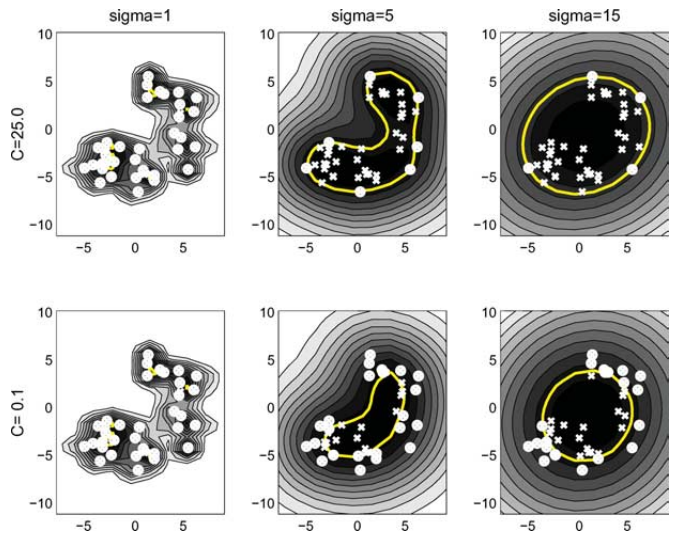
\includegraphics[scale=0.6]{Imgs/svdd1.png}
\caption{توصیف‌گر آموزش دیده بر روی یک مجموعه‌داده تست با استفاده از یک تابع هسته گاوسی با واریانس‌های مختلف و به ازای دو مقدار متفاوت پارامتر $C$. بردارهای پشتیبان با دایره‌های سفید و محدوده تخمین‌ زده شده برای داده‌ها با خط زرد مشخص شده‌اند \cite{tax2004support}.}
\label{fig:1}
\end{figure*}

همین‌طور شعاع محدوده داده‌ها را می‌توان با استفاده از رابطه \eqref{eq:10} محاسبه نمود که در آن $x_k$ می‌تواند هر یک از بردارهای پشتیبان باشد.
\begin{align*}
R^2 &= (x_k\cdot x_k)-2\mathlarger{\Sigma_i}\alpha_i (x_k \cdot x_i) \\&+ \mathlarger{\Sigma_{ij}} \alpha_i \alpha_j (x_i \cdot x_j)
\numberthis 
\label{eq:10}
\end{align*}
شایان ذکر است که مطابق با پژوهش .vapnik... به جای تمامی ضرب‌های داخلی می‌توان از توابع هسته مختلفی استفاده نمود که در بالابردن قدرت مدل نقش مهمی را ایفا می‌کنند. شکل 
\ref{fig:1}
عملکرد الگوریتم ارائه شده را با استفاده از یک تابع هسته گاوسی با واریانس‌های مختلف، نمایش می‌دهد. همان‌طور که در شکل مشخص است،‌ با افزایش مقدار پارامتر $C$ میزان سخت‌گیری روش در محدودیت شمول افزایش می‌یابد و داده‌های بیشتری در محدوده تخمین‌ زده شده الگوریتم قرار می‌گیرند.

\section{ماشین بردار پشتیبان خطی}


\bibliographystyle{ieeetr}
\bibliography{ref}

\end{document} 
